\section{Propagation Equation and Population Rate Equations}

The electric field is written as a carrier wave modulated by a slowly varying envelope $u(r,t,z)$, and the wave equation is reduced under the slowly varying envelope approximation. For fused silica, the resulting propagation equation used in the code reads:
\begin{align}
\label{eq:master_propagation}
\hat{U}\,\frac{\partial u}{\partial z} =\;
&\underbrace{\frac{i}{2k_0}\nabla_\perp^2 u}_{\text{diffraction}}
\;+\;
\underbrace{i\,\hat{D}\,\hat{U}\,u}_{\substack{\text{dispersion: exact Sellmeier, all orders}\\
\text{leading term } -\tfrac{i}{2}k''_\omega\,\partial_t^2 u}} \nonumber\\[4pt]
&+\;\underbrace{i\,\hat{T}^{2}\,\frac{3\omega_0^2\chi^{(3)}}{8k_0c^2}(1-f_R)\,|u|^2\,u}_{\text{instantaneous Kerr effect and self-steepening}} \nonumber\\[4pt]
&+\;\underbrace{i\,\hat{T}^{2}\,\frac{3\omega_0^2\chi^{(3)}}{8k_0c^2}\,f_R\,\big(R * |u|^2\big)\,u}_{\text{delayed Raman response}} \nonumber\\[4pt]
&-\;\underbrace{\hat{T}\,\frac{U_i\,W_{PI}(|u|)}{n_0c\varepsilon_0|u|^2}\left(1-\frac{N}{N_{at}}\right)u}_{\text{photoionization energy loss}}
\;-\;\underbrace{\frac{\sigma_\omega}{2}\big(1+i\omega_0\tau_c\big)N\,u}_{\text{plasma absorption and defocusing}} \nonumber\\[4pt]
&+\;\underbrace{i\,\frac{\omega_0}{2n_0c\,\rho_c}\frac{\omega_0^2}{\omega_{tr}^2-\omega_0^2}\,N_{STE}\,u}_{\text{bound STE polarizability, new in Section~11.4}}
\end{align}

with, in the retarded frame $t\to t-z/v_g$ and writing $\Omega=\omega-\omega_0$,
\begin{equation}
\hat{T} = 1+\frac{i}{\omega_0}\frac{\partial}{\partial t} \;\longleftrightarrow\; 1+\frac{\Omega}{\omega_0},
\qquad
\hat{U} = 1+\frac{i k'_\omega}{k_0}\frac{\partial}{\partial t} \;\longleftrightarrow\; 1+\frac{k'_\omega\Omega}{k_0},
\end{equation}
\begin{equation}
\hat{D} \;\longleftrightarrow\; k(\omega)-k_0-k'_\omega\Omega ,
\end{equation}
where $k(\omega)$ is evaluated from the Sellmeier relation rather than truncated at any order.

This is the form used by Couairon et al.~\cite{PhysRevB.71.125435}, whose Eq.~(2) is introduced with exactly that wording: the equation accounts for space-time focusing \emph{due to the presence of the operator $\hat{U}$ in front of $\partial/\partial z$}. The reason to prefer it over the algebraically equivalent form obtained by dividing through by $\hat{U}$ is that it contains no inverse operator, so there is no ambiguity about which terms $\hat{U}$ acts on. If one does divide by $\hat{U}$, it must be applied to \emph{every} term on the right-hand side, giving
\begin{equation}
\label{eq:master_divided}
\frac{\partial u}{\partial z} = \frac{i}{2k_0}\hat{U}^{-1}\nabla_\perp^2 u + i\hat{D}u
 + \hat{U}^{-1}\Big\{\text{Kerr} + \text{Raman} + \text{ionization} + \text{plasma} + \text{STE}\Big\},
\end{equation}
where $\hat{U}$ cancels on the dispersion term alone. Since $\hat{U}\simeq\hat{T}$ to within one percent for fused silica at $800\ \text{nm}$ ($n_g/n_0=1.0095$), the Kerr operator in that form becomes $\hat{U}^{-1}\hat{T}^2\simeq\hat{T}$ and the ionization operator becomes $\hat{U}^{-1}\hat{T}\simeq1$, which is how the single-$\hat{T}$ expressions of the review literature arise. Applying $\hat{U}^{-1}$ to the Laplacian only, while leaving $\hat{T}^2$ on the Kerr term, is \emph{not} one of these two forms and leaves every nonlinear term with one power of $\hat{T}$ too many.

Second, the depletion factor is the dimensionless $1-N/N_{at}$, not $N_{at}-N$. The Keldysh rate $W_{PI}$ returned by the lookup table is already a volumetric rate in $\text{cm}^{-3}\text{s}^{-1}$, so multiplying it by a density would leave the term with an extra $\text{cm}^{-3}$. The alternative convention, in which $W_{PI}$ is a per-atom rate in $\text{s}^{-1}$ multiplied by $N_{at}-N$, is equally valid but is not the quantity the code computes.

Third, the group delay $k'_\omega\Omega$ does not appear as a separate term: it has been absorbed into $\hat{D}$, because the code works in the retarded frame and subtracts it inside \texttt{delta\_k}. Writing it again outside would count it twice.

\paragraph{How the solver implements this.} Equation~\eqref{eq:master_propagation} cannot be stepped forward as written, since it gives $\hat{U}\partial_z u$ rather than $\partial_z u$; the code therefore integrates the divided form~\eqref{eq:master_divided}. The linear half step supplies the first two terms, applying \texttt{inv\_U\_op} to the Laplacian and leaving \texttt{delta\_k} bare, and the nonlinear step assembles the whole brace in frequency space and multiplies it by $\hat{U}^{-1}$ in one operation, so that the Kerr, Raman, ionization, plasma and STE terms all receive it. Because $\hat{U}^{-1}$ here multiplies source terms directly rather than sitting inside a phase factor $e^{i\varphi}$, it is floored and masked before use: $\hat{U}$ vanishes at $\Omega=-k'_\omega{}^{-1}k_0\simeq-0.99\,\omega_0$, that is at essentially zero absolute frequency. The floor only acts beyond $\lambda=7.4\ \mu\text{m}$, outside the Sellmeier window where the spectral mask has already suppressed the field, so within the physical band $\hat{U}^{-1}$ stays between $0.22$ and $6.6$ and is not distorted.

\subsection{Where the Self-Steepening Operator Comes From, and Why It Is Squared on Some Terms}

Section~6 introduced self-steepening through the time domain shock term $(2n_2/c)\,\partial(|\mathcal{E}|^2\mathcal{E})/\partial t$. The propagation equation above instead writes it as a frequency domain multiplication by $T=1+\Omega/\omega_0$, or $T^2$ on some terms. These are the same physics in two different languages, and the reason some terms get $T$, some get $T^2$, and the plasma term gets no such operator at all, comes directly from how many time derivatives that term carries before the slowly varying envelope approximation is applied.

Every source term on the right hand side of the underlying wave equation originates from a current or a polarization evaluated at the true, unapproximated frequency $\omega=\omega_0+\Omega$ of each spectral component, not at the fixed carrier frequency $\omega_0$. Writing $\omega=\omega_0(1+\Omega/\omega_0)=\omega_0T$, any factor of $\omega$ appearing in a source term becomes a factor of $\omega_0T$ once it is pulled out and referenced to the carrier frequency, exactly as $k(\omega)$ was expanded around $k_0$ for the dispersion term. The Kerr polarization enters the wave equation through $\partial^2P_{NL}/\partial t^2$, a second time derivative, which in the frequency domain is a factor of $-\omega^2=-\omega_0^2T^2$. The photoionization current, like the plasma current, enters through a single time derivative $\partial J/\partial t$, a factor of $-i\omega=-i\omega_0T$. This is the entire reason the Kerr and Raman terms above carry $T^2$ while the photoionization loss term carries only $T$. Both are the same operator $T=1+\Omega/\omega_0$, applied once for every power of $\omega$ that the term's own derivation contributes, and Section~11.4 of \texttt{deliverable~(3)} corrects the July code precisely because it had applied $T$ to the Kerr term as if it only carried one such derivative.

The plasma current $J_{plasma}$ also comes from a single time derivative, so by the same counting it should carry $T^1$ as well. It appears without any $T$ in the equation above because the Drude derivation of Section~7 already keeps the full frequency dependence of $\sigma(\omega)$ and $(1+i\omega\tau_c)$ exactly, rather than expanding around $\omega_0$ first, so the correction is already built into $\sigma_\omega$ itself and does not need to be reintroduced as a separate multiplicative operator.

Physically, $T$ being larger than one on the blue side of the spectrum ($\Omega>0$) and smaller than one on the red side is exactly the same statement as the shock term of Section~6 pulling energy toward the trailing edge of the pulse: whichever nonlinear term this operator multiplies, it systematically favors the blue shifted, trailing part of the spectrum over the red shifted, leading part, which is the frequency domain signature of the group velocity depending on intensity. Squaring the operator on the Kerr term simply means this asymmetry is applied twice, once for each power of $\omega$ that the second time derivative of $P_{NL}$ contributes, and is why the Kerr induced spectral asymmetry is normally the dominant contribution to self-steepening compared to the single power of $T$ on photoionization loss.

Each underbraced term maps onto a specific piece of the code. Diffraction and dispersion are applied together by \texttt{LinearOperator.half\_linear}, in the quasi discrete Hankel basis described in Section~12. They are combined into a single step rather than split into two because both are diagonal once expressed in (Hankel radial mode, temporal frequency $\Omega$) space, so they commute and applying them together is exact, at the cost of one FFT/IFFT pair per call instead of two. The space-time focusing factor enters this same step as \texttt{inv\_U\_op} $=1/\hat{U}(\Omega)$ multiplying the transverse Laplacian, and reduces to the identity when \texttt{enable\_space\_time\_focusing} is off. Rather than truncating the Taylor expansion of $k(\omega)$ at second order as we did analytically in the derivation of Section~6, the code evaluates $k(\omega)$ directly from the Sellmeier relation for every frequency component and subtracts the linear term $k_0+k'_\omega\Omega$, so the operator \texttt{delta\_k} used in the code already contains dispersion to all orders, not just group velocity dispersion.

The Kerr, self-steepening, and Raman terms are computed together in \texttt{NonlinearOperator.split}. The instantaneous part $(1-f_R)|u|^2$ and the delayed Raman part $f_R\,(R * |u|^2)$, obtained by convolving the intensity with the retarded Raman response function $R(t)$, are summed before multiplying by $u$, which is why they are written here as two separate lines rather than as two independent physical effects. The self-steepening operator $\big(1+\tfrac{i}{\omega_0}\partial_t\big)$ is applied in the frequency domain as \texttt{T\_op} $= 1+\Omega/\omega_0$, following the same operator introduced by Mao et al.~\cite{mao2004} for free carrier absorption and used identically here for the Kerr response.

The photoionization loss term removes energy from the field at exactly the rate needed to promote electrons to the conduction band at the Keldysh rate $W_{PI}$, throttled by the fraction $1-N/N_{at}$ of ionizable sites still neutral, consistent with the ionization loss derivation of Section~11.3 below. $N_{at}$ is the total density of ionizable sites (\texttt{rho\_max} in the code) and $N$ is the current free electron density; in the code this factor is \texttt{depl\_field = clip(1 - rho/rho\_max, 0, 1)}. The plasma absorption and plasma induced defocusing are grouped into a single term above since the code computes them together as the real and imaginary parts of the same Drude response derived in Section~7, with $\sigma_\omega$ the inverse Bremsstrahlung cross section already introduced in Section~5.

\authornote{The Raman response function $R(t)$ used in the code, with time constants \texttt{tau\_s} and \texttt{tau\_d}, is the standard damped oscillator form used for silica nonlinear optics. If you want the explicit derivation of $R(t)$ from a driven harmonic oscillator model included here, let me know and I will add it with the matching reference.}

\paragraph{Update relative to the July solver (\texttt{deliverable~(3)}).} Eq.~(4) of Couairon et al.~\cite{PhysRevB.71.125435} squares the self-steepening operator on the Kerr and Raman terms, $\big(1+\tfrac{i}{\omega_0}\partial_t\big)^2$, applies it only to the first power on the photoionization loss term, and applies none at all to the plasma term. The July code in \texttt{NewSim3juillet.py} used a single \texttt{T\_op} on both the Kerr and the photoionization terms, and \texttt{deliverable~(3)} initially changed this to \texttt{T\_op**2} on the Kerr term to match the paper.

That change, taken alone, was a regression, and it is worth recording why because the reasoning looks sound. Couairon's $\hat{T}^2$ lives in his Eq.~(2), which carries $\hat{U}$ in front of $\partial/\partial z$; the July code had no $\hat{U}$ anywhere, so its single $\hat{T}$ was already the correct value of $\hat{U}^{-1}\hat{T}^2$ for a model without space-time focusing. Importing the numerator of one form while keeping the left-hand side of the other left the self-steepening roughly twice too strong: expanding in $\varepsilon=\Omega/\omega_0$ gives $\hat{T}^2=1+2\varepsilon+\varepsilon^2$ against the correct $\hat{U}^{-1}\hat{T}^2=1+0.99\,\varepsilon$, and since self-steepening \emph{is} the departure from unity, the modelled effect was doubled at leading order, rising to a factor of three on the far blue wing. The present version resolves this by applying $\hat{U}^{-1}$ to the entire nonlinear bracket, as described above, which reproduces Eq.~(2) exactly rather than approximately and, unlike the shortcut of simply reverting the Kerr term to $\hat{T}^1$, also supplies the $\hat{U}^{-1}$ that the plasma and STE terms require. The solver keeps the spectral mask \texttt{spec\_mask} multiplying \texttt{T\_op}, since $T=1+\Omega/\omega_0$ becomes negative for absolute frequencies below zero and this sign flip was found to be numerically unstable, amplified by up to a factor $9$ per step once the operator is squared. The mask is a smooth tanh window that suppresses the field outside the wavelength range where the Sellmeier fit is valid, $\lambda\in[0.18,5]\ \mu\text{m}$, and is controlled by \texttt{enable\_spectral\_filter}, default on. It has no effect on the physical, non-negative-frequency part of the spectrum. Six new boolean switches, one per term of the equation above (instantaneous Kerr, Raman, self-steepening, photoionization loss, plasma defocusing, plasma absorption, named \texttt{enable\_kerr\_instantaneous} through \texttt{enable\_plasma\_absorption} in the code), were also added so each term can be switched off independently. This is what the ablation study of the accompanying notebook uses to test what every term actually does to the beam rather than only reading it from the equation.

\subsection{Carrier Density Rate Equations}

The code integrates two coupled populations, the free electron density $N$ and the self-trapped exciton density $N_{STE}$, exactly as introduced in Section~5:
\begin{align}
\frac{dN}{dt} =\;
&\underbrace{W_{PI}(|u|)\,(N_{at}-N)}_{\text{direct photoionization, depletes available sites}} \nonumber\\[4pt]
&+\;\underbrace{\Big[W_{PI}(|u_x|)+\beta_s I\, N\Big]\frac{N_{STE}}{N_{at}}}_{\text{re-ionization of trapped excitons}} \nonumber\\[4pt]
&+\;\underbrace{\frac{\sigma_\omega}{U_i} I\, N\,(1-N/N_{at})}_{\text{avalanche ionization}}
\;-\;\underbrace{\frac{N}{\tau_r}}_{\text{trapping into the STE channel}}
\end{align}
\begin{align}
\frac{dN_{STE}}{dt} =\;
&\underbrace{\frac{N}{\tau_r}}_{\text{trapping}}
\;-\;\underbrace{\Big[W_{PI}(|u_x|)+\beta_s I\, N\Big]\frac{N_{STE}}{N_{at}}}_{\text{re-ionization}}
\end{align}
where $I=n_0c\varepsilon_0|u|^2/2$ is the local intensity, $u_x$ is the field evaluated with the smaller gap $U_s$ of the trapped state instead of $U_i$, so that $W_{PI}(|u_x|)$ is the Keldysh rate computed for the shallower STE gap, and $\beta_s$ is the avalanche coefficient for the STE channel. This two population model with a distinct gap $U_s$ for the trapped state follows the parametrization used in the code (\texttt{Us\_eV}, labeled Chimier PRB 2011 in the source comments).

\authornote{I have not been able to check this rate equation against the original Chimier, PRB 84, 075092 (2011) paper, since it is not among the sources currently in the repository. If you upload it, I will verify the coefficients $\beta_s$ and $U_s$ against it directly and correct this section if needed.}

\begin{figure}[htbp]
    \centering
    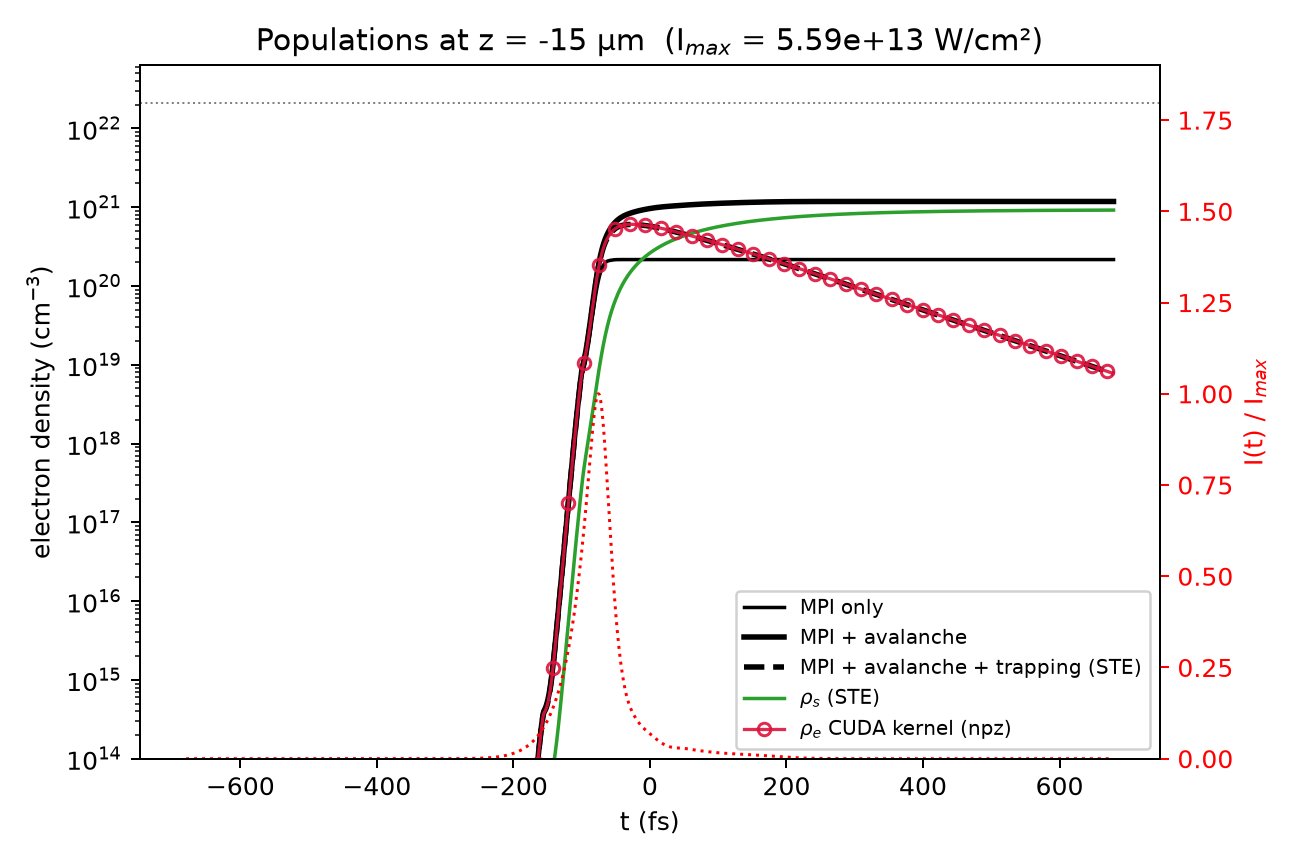
\includegraphics[width=0.85\linewidth]{fig2_populations.png}
    \caption{On-axis electron populations at the nonlinear focus for the $800\ \text{nm}$, $1.1\ \mu$J experiment of Fig.~\ref{fig:fig8_peak_intensity}, reintegrating the 0D rate equations above from the saved intensity trace $I(t)$ under three models (MPI only, $+$avalanche, $+$avalanche$+$trapping) and superposing the actual $N(t)$ the CUDA kernel computed on-axis (open circles). The full model coincides with the CUDA output by construction, which is what this overlay is meant to check, and the agreement confirms the exponential-integrator time stepping of Section~12 reproduces the same rate equations solved here analytically term by term. Trapping into $N_{STE}$ (green) becomes the dominant channel within a few hundred femtoseconds of the pulse peak, draining $N$ (dashed black) down from its avalanche-augmented maximum, consistent with the trapping time $\tau_r$ used throughout this report.}
    \label{fig:fig2_populations}
\end{figure}

\begin{figure}[htbp]
    \centering
    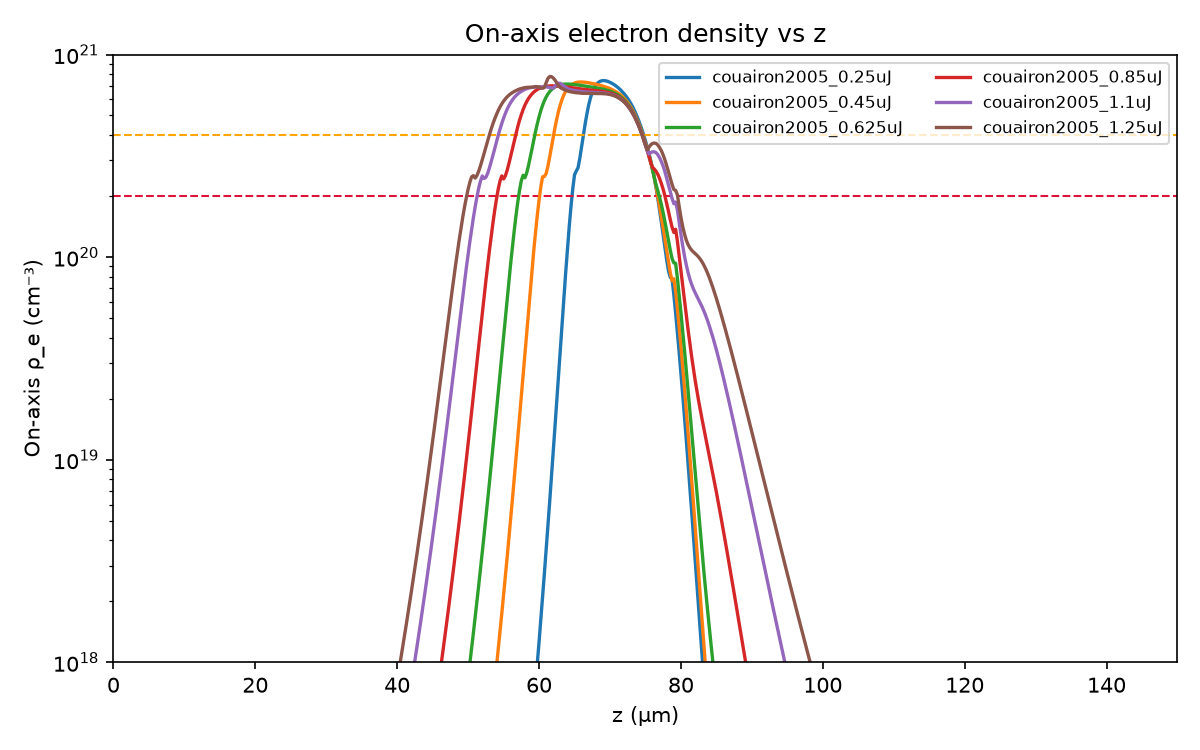
\includegraphics[width=0.85\linewidth]{couairon2005_fig9_energy_sweep.png}
    \caption{On-axis electron density along $z$ for the same six input energies as Fig.~\ref{fig:fig8_peak_intensity}, reproducing Fig.~9 of~\cite{PhysRevB.71.125435}. The dashed lines mark $1$ and $2\times10^{20}\ \text{cm}^{-3}$ as reference levels. As with the peak intensity, every above-threshold curve saturates near a common density once the local intensity reaches $I_{clamp}$, the electron-density signature of the same clamping balance seen in Fig.~\ref{fig:fig8_peak_intensity}.}
    \label{fig:fig9_energy_sweep}
\end{figure}

\begin{figure}[htbp]
    \centering
    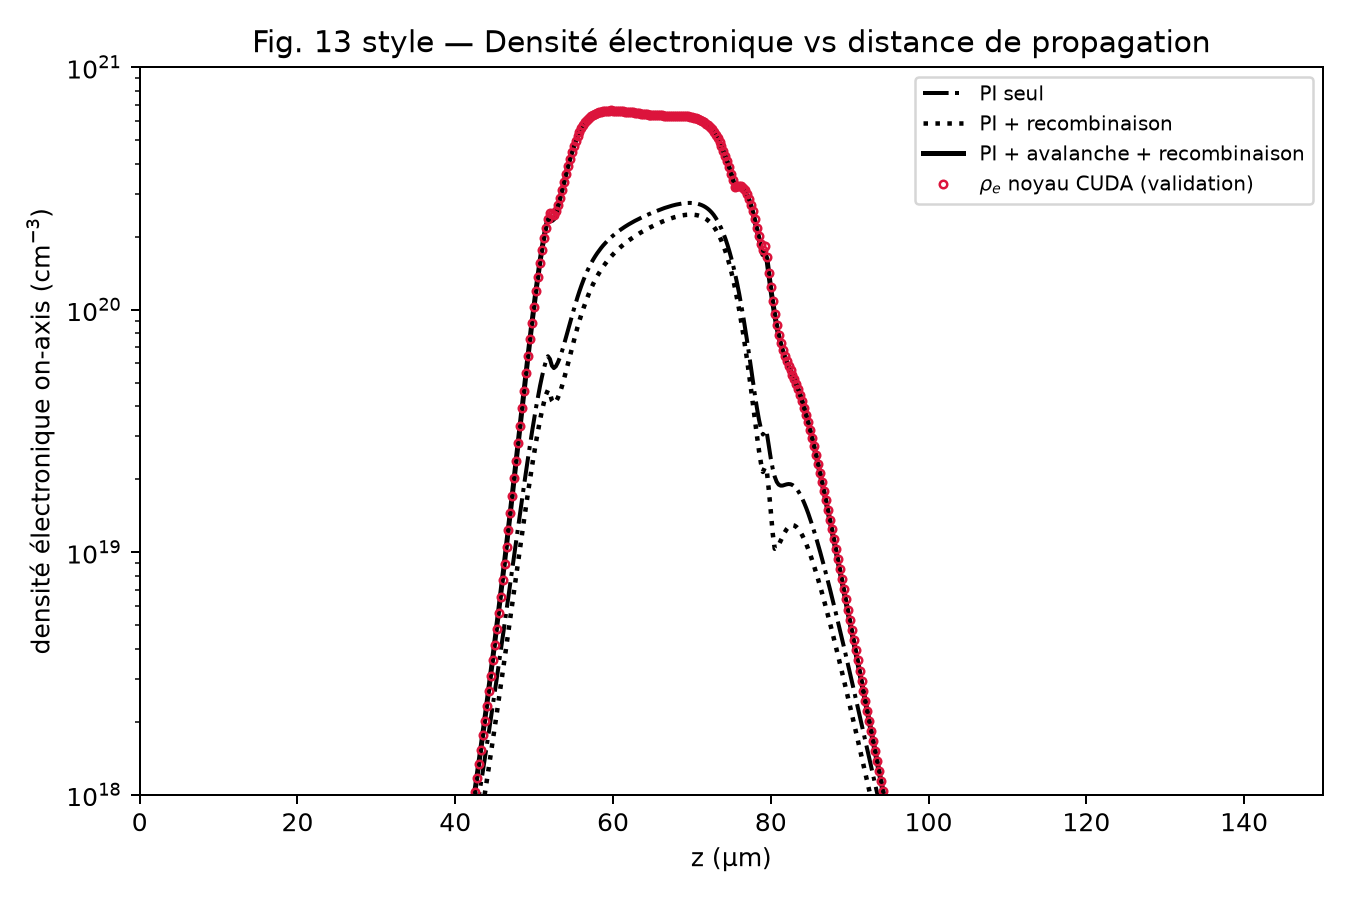
\includegraphics[width=0.85\linewidth]{fig13_electron_density_vs_z.png}
    \caption{On-axis electron density along $z$ at fixed input energy ($1.1\ \mu$J), comparing PI only, PI$+$recombination and PI$+$avalanche$+$recombination against the CUDA kernel output (open circles), reproducing Fig.~13 of~\cite{PhysRevB.71.125435}. The full model (thick solid) tracks the CUDA output essentially exactly across the four decades shown, while PI-only and PI$+$recombination without avalanche fall visibly below it on the upstream side of the profile (smaller $z$, before the nonlinear focus), isolating the specific contribution of the avalanche term of Eq.~\eqref{eq:master_propagation}, $\sigma_\omega I N/U_i$, to the total carrier yield.}
    \label{fig:fig13_electron_density}
\end{figure}

Note the correspondence with Section~5. There, we wrote the same pair of equations with $\sigma/E_g$ in place of $\sigma_\omega/U_i$ and $\tau_x$ in place of $\tau_r$. These are the same quantities, only the notation has been aligned here with the variable names used in the code (\texttt{tau\_r} for the trapping time, \texttt{avalanche\_coef} for $\sigma_\omega/U_i$).

\paragraph{Update relative to the July solver.} The July code only let the self-trapped exciton population decay by re-ionization back into the conduction band, the $\big[W_{PI}(|u_x|)+\beta_sIN\big]N_{STE}/N_{at}$ term above. The parametrization referenced in the code (Sakurai et al.) tabulates for fused silica both a trapping time of $150\ \text{fs}$, already present as $\tau_r$, and a separate relaxation time of the trapped state itself of about $1\ \text{ps}$, which was missing. \texttt{deliverable~(3)} adds an optional term $-N_{STE}/\tau_{STE}$ to the $dN_{STE}/dt$ equation, controlled by \texttt{Config.tau\_ste}, defaulting to \texttt{None} which reproduces the July behavior exactly. This mainly matters for the probe phase at picosecond delays, since it changes how long the STE population, and therefore the index change it produces (Section~11.4), survives after the pump pulse has left.

\subsection{Photoionization Energy Loss}

For completeness we derive the photoionization loss term used above, since it does not appear explicitly in the earlier sections. Each ionization event removes one photoelectron from the neutral population and costs at least the gap energy $U_i$, which is taken directly from the field. The absorbed power per unit volume is:
\begin{equation}
\mathcal{P}_{ion} = U_i\,(N_{at}-N)\,W_{PI}(|u|)
\end{equation}
Writing this as a loss term $-\alpha_{ion}I$ acting on the intensity $I=n_0c\varepsilon_0|u|^2/2$ and solving for $\alpha_{ion}$ gives the coefficient used above:
\begin{equation}
\alpha_{ion} = \frac{U_i\,(N_{at}-N)\,W_{PI}(|u|)}{n_0c\varepsilon_0|u|^2/2}
\end{equation}
which is exactly the \texttt{photo} variable computed inside \texttt{NonlinearOperator.split}.

\subsection{Bound Polarizability of Self-Trapped Excitons}

This subsection documents a term that did not exist at all in the July solver and is new in \texttt{deliverable~(3)}. A self-trapped exciton is not a conduction band carrier. It is a pair of dangling bonds, $\text{Si}^\bullet$ and $\text{O}^\bullet$, left behind after the Si-O-Si bond breaks, described in Section~10, and its unpaired orbitals sit inside the gap rather than in the conduction band. It therefore does not drift in the field and does not contribute to the free carrier Drude response of Section~7. What it does instead is polarize as a bound oscillator with a resonance at the energy of its first excited level, following Mao et al.~\cite{mao2004}:
\begin{equation}
\Delta n_{STE} = \frac{N_{STE}\,e^2}{2n_0m_e\varepsilon_0}\,\frac{1}{\omega_{tr}^2-\omega^2}
\end{equation}
The July code, and the interferometry section of this report, only ever evaluated this formula for the probe beam in post-processing, in \texttt{unified\_filament\_slider\_v3.py}. It never entered the propagation equation itself, so the pump pulse never felt the index change its own trapped population produces. \texttt{deliverable~(3)} adds this contribution directly to the field equation as the fifth line above, controlled by \texttt{enable\_ste\_index}, default on, and implemented as a pure phase term with no associated loss, since the pump photon energy at $1.55\ \text{eV}$ is far from the STE resonance, so there is no one-photon absorption to account for on the pump itself. Because the pump lies below the resonance, $\omega_0<\omega_{tr}$, this term is positive and adds to the Kerr self-focusing rather than opposing it, which is also the mechanism identified as the permanent, fracture-free index change that Couairon et al. classify as type I damage.

A second correction accompanies this addition. The resonance energy itself was taken as $5.2\ \text{eV}$ in the July code, but Mao et al. specify $5.2\ \text{eV}$ as the peak of the STE transient absorption band, not the resonance frequency to use for the refractive index formula above, for which they give the first excited level at $\omega_{tr}\approx 4.2\ \text{eV}$. \texttt{deliverable~(3)} corrects \texttt{E\_tr\_eV} to $4.2$, which changes the resonance denominator at the $490\ \text{nm}$ probe wavelength used in this report by a factor of about $1.84$.

\authornote{I have not independently re-derived the bound oscillator formula for $\Delta n_{STE}$ from first principles here, I have only checked that the code matches the Mao et al. expression term for term. If you want the Lorentz oscillator derivation included for completeness, let me know.}
